\documentclass[hidelinks,12pt]{article}

\usepackage[brazil]{babel}
\usepackage[utf8]{inputenc}
\usepackage{amsmath}
\usepackage{amsfonts}
\usepackage{amssymb}
\usepackage{indentfirst}
\usepackage{color}
\usepackage{mathrsfs}
\usepackage{pgfplots}
\usepackage{hyperref}
\usepackage{fancyhdr}
\usepackage{graphicx}
\usepackage[export]{adjustbox}
\newcommand{\icon}[1]{\includegraphics[height=12pt]{#1}}
\newcommand{\bigicon}[1]{\includegraphics[height=50pt]{#1}}

\newcommand{\iconb}[1]{\includegraphics[height=20pt]{#1}}
\setcounter{secnumdepth}{5}

\fancypagestyle{plain}{%
	\fancyfoot{}%
	\fancyhead{}%
}


\begin{document}
\pagenumbering{gobble}
\pagestyle{fancy}


\lhead{\bigicon{Figures/ufu}}
\chead{{\footnotesize UNIVERSIDADE FEDERAL DE UBERLÂNDIA \\ FACULDADE DE CIÊNCIA DA COMPUTAÇÃO \\ Inteligência Computacional} \\ \scriptsize{Av. João Naves de Ávila 2121, Campus Santa Mônica} }
\rhead{\bigicon{Figures/facom}}
\lfoot{}
\cfoot{}
\rfoot{}
\vspace*{10cm}
\begin{figure}[!h]
	\centering
	\Huge{Inteligência Coletiva}
\end{figure}

\vspace{5cm}
\noindent\textbf{Aluno:} Leonardo da Silva Martins - 11321BCC034\\
\textbf{Prof.:} Gina


\newpage
\fancyhead[C]{}
\fancyhead[R]{}
\fancyhead[L]{\leftmark}
\fancyfoot{}
\fancyfoot[L]{{\footnotesize  Inteligência Computacional}}
\fancyfoot[C]{\hspace{1.5cm}\thepage}
\fancyfoot[R]{{\footnotesize Inteligência Coletiva}}
\pagenumbering{arabic}


\tableofcontents

{\let\thefootnote\relax\footnotetext{\textit{UFU, Universidade Federal de Uberlândia, Minas Gerais, Brasil}}}

\newpage

\section{Introdução}

    Estre relatório apresenta as resoluções dos exercícios do problema do caixeiro viajante, utilizando o algoritmo de colônia de formigas, propostos no trabalho sobre Inteligência Coletiva da disciplina de Inteligência Computacioanl.

\section{Metodologia}
	
	Neste trabalho utilizamos a estrutura de matriz para representar as tabelas utilizadas, como tabela de probabilidade, tabela de distâncias, tabela de feromônio entre outras, onde a relação entre a linha i e a coluna j representa a relação entra a cidade i e a cidade j.

\section{Problema do Caixeiro Viajante}
	
	O problema do caixeiro viajante (PCV ou TSP – Traveling Salesman Problem) é assim definido: dado um número finito de cidades e o custo de viagem entre cada par, deve-se encontrar o caminho que passa por todas as cidades e retorna para o ponto inicial com custo mínimo, passando por cada cidade apenas uma vez. Embora seja simples de definir, o TSP é um problema combinatório clássico comprovadamente NP-Difícil com aplicações nas áreas de logística, genética, telecomunicações e neurociência, entre outras.	 
		
\section{Exercícios}

	Seguem as respostas para os exercícios referentes ao trabalho, onde iremos mudar os seguintes fatores para cada experimento.
	
	\begin{itemize}
		\item Número de repetições
		\item Número máximo de iterações para achar o melhor caminho
		\item Quantidade de feromôneo depositado por cada formiga
		\item Taxa de evaporação do feromônio
	\end{itemize}

	
	\subsection{M6}
			Neste exercício é fornecido uma matriz de distância entre 6 cidades diferentes.	
		\subsubsection{Primeira configuração}
		 	Para este experimento foi utilizada a seguinte configuração:

		 	\begin{itemize}
				\item Número de repetições: 50
				\item Número máximo de iterações para achar o melhor caminho: 100
				\item Quantidade de feromôneo depositado por cada formiga: 1
				\item Taxa de evaporação do feromônio: 0.5
			\end{itemize}

		\newpage			
			
		\begin{figure}[!h]
			\centering
			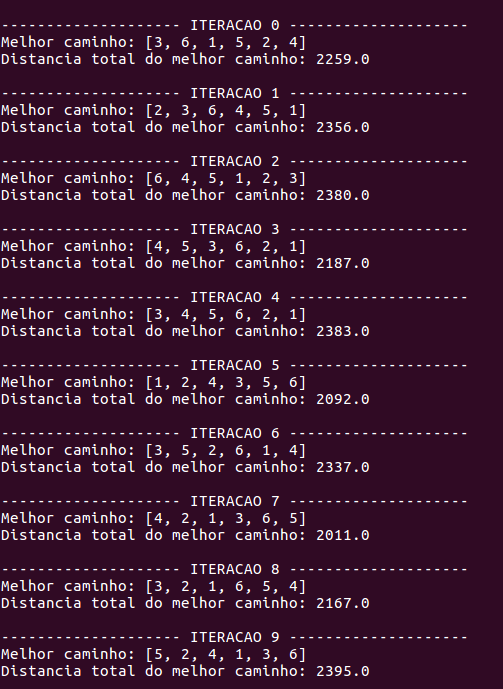
\includegraphics[scale=0.6]{Figures/m6-1-1.png}
		\end{figure}

		\newpage

		\begin{figure}[!h]
			\centering
			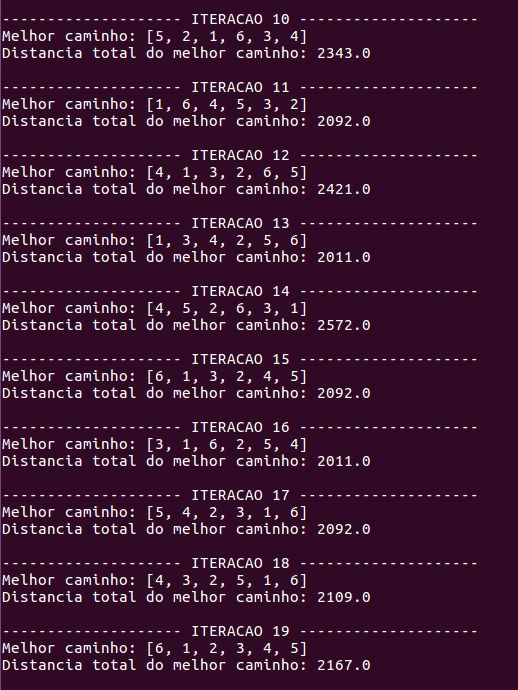
\includegraphics[scale=0.6]{Figures/m6-1-2.png}
		\end{figure}

		\newpage

		\begin{figure}[!h]
			\centering
			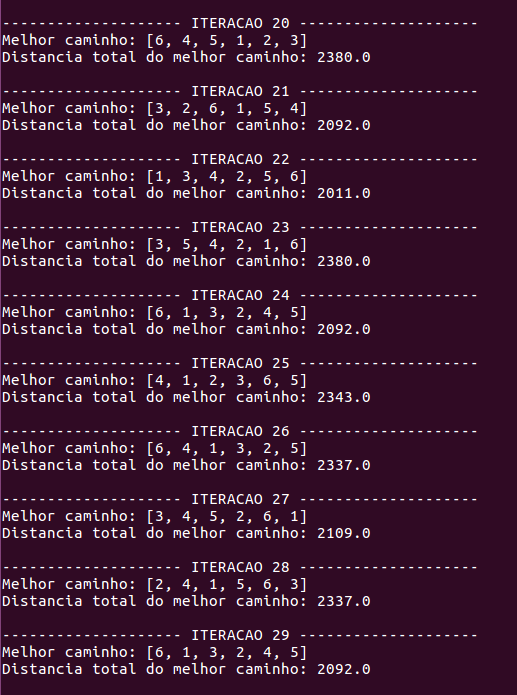
\includegraphics[scale=0.6]{Figures/m6-1-3.png}
		\end{figure}

		\newpage

		\begin{figure}[!h]
			\centering
			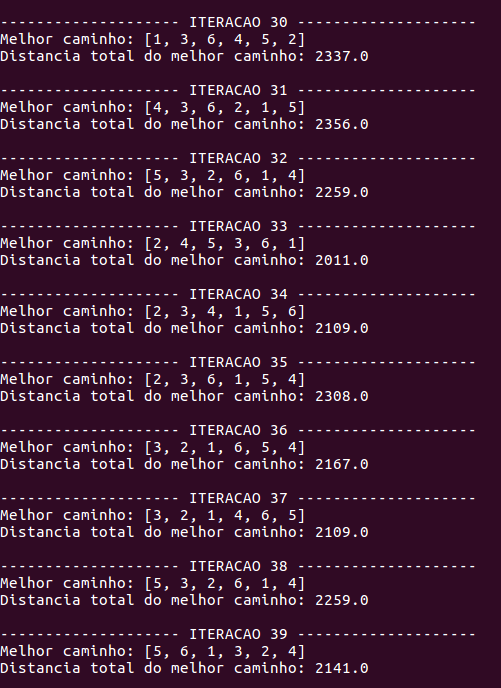
\includegraphics[scale=0.6]{Figures/m6-1-4.png}
		\end{figure}

		\newpage

		\begin{figure}[!h]
			\centering
			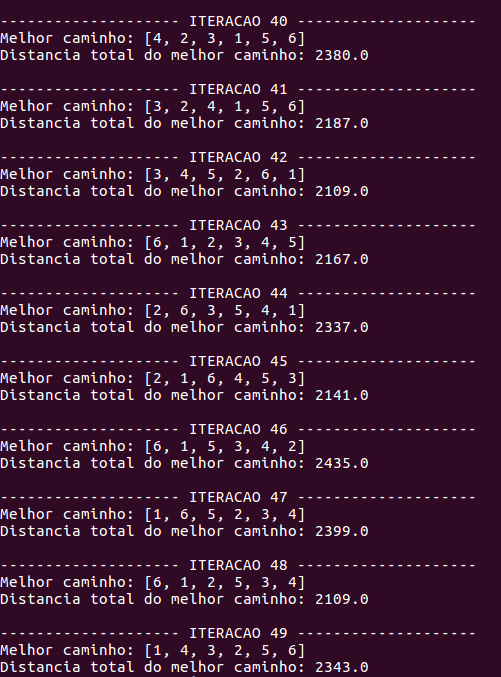
\includegraphics[scale=0.6]{Figures/m6-1-5.png}
		\end{figure}
		
		\newpage
		
		\subsubsection{Segunda configuração}
		 	Para este experimento foi utilizada a seguinte configuração:

		 	\begin{itemize}
				\item Número de repetições: 50
				\item Número máximo de iterações para achar o melhor caminho: 1000
				\item Quantidade de feromôneo depositado por cada formiga: 1
				\item Taxa de evaporação do feromônio: 0.8
			\end{itemize}

		\newpage
			
		\begin{figure}[!h]
			\centering
			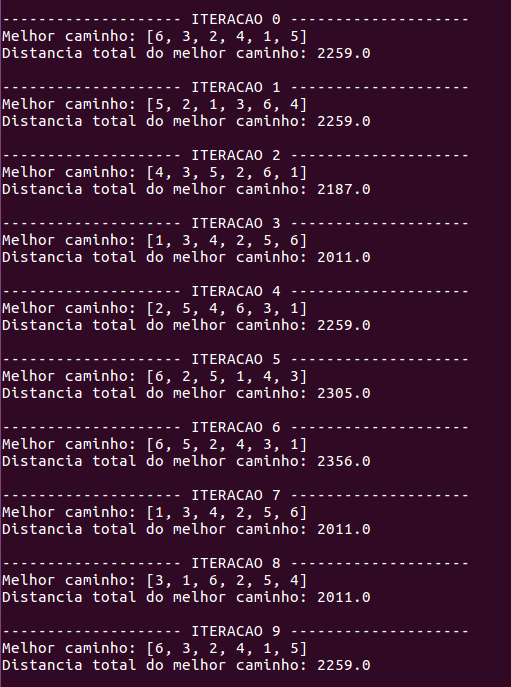
\includegraphics[scale=0.6]{Figures/m6-2-1.png}
		\end{figure}

		\newpage

		\begin{figure}[!h]
			\centering
			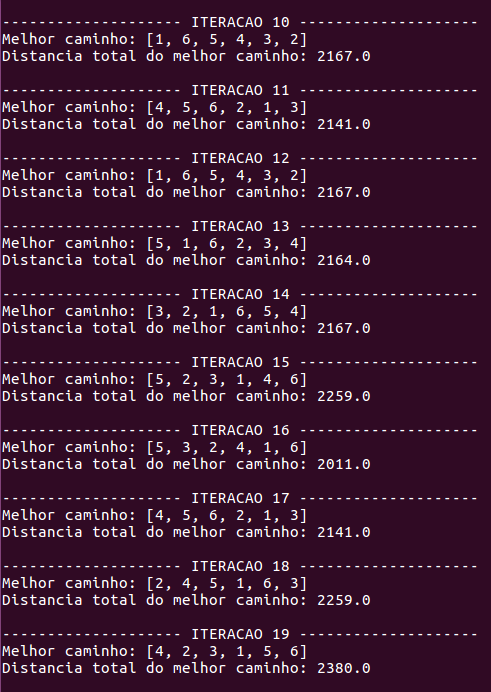
\includegraphics[scale=0.6]{Figures/m6-2-2.png}
		\end{figure}

		\newpage

		\begin{figure}[!h]
			\centering
			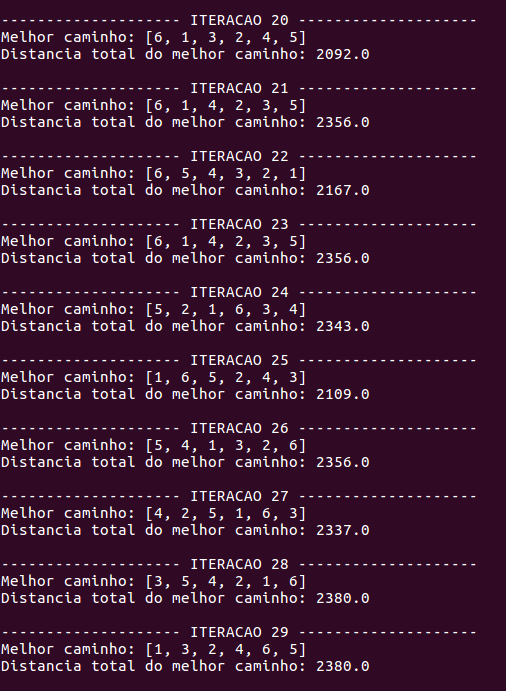
\includegraphics[scale=0.6]{Figures/m6-2-3.png}
		\end{figure}

		\newpage

		\begin{figure}[!h]
			\centering
			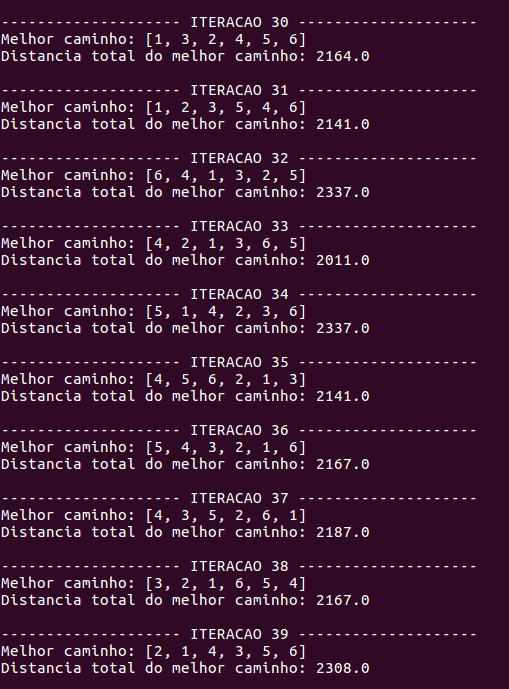
\includegraphics[scale=0.6]{Figures/m6-2-4.png}
		\end{figure}

		\newpage

		\begin{figure}[!h]
			\centering
			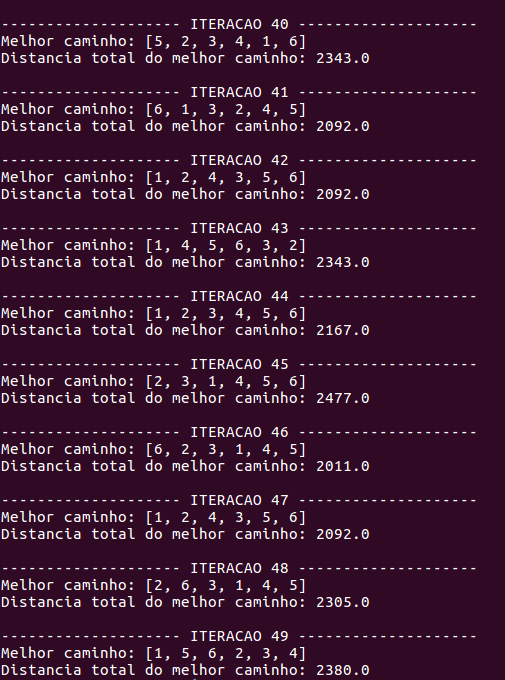
\includegraphics[scale=0.6]{Figures/m6-2-5.png}
		\end{figure}

		\newpage

	
	\subsection{M15}
			Neste exercício é fornecido as coordenadas de 15 cidades diferentes.	
		\subsubsection{Primeira configuração}
		 	Para este experimento foi utilizada a seguinte configuração:

		 	\begin{itemize}
				\item Número de repetições: 50
				\item Número máximo de iterações para achar o melhor caminho: 100
				\item Quantidade de feromôneo depositado por cada formiga: 1
				\item Taxa de evaporação do feromônio: 0.5
			\end{itemize}

		\newpage	

		\begin{figure}[!h]
			\centering
			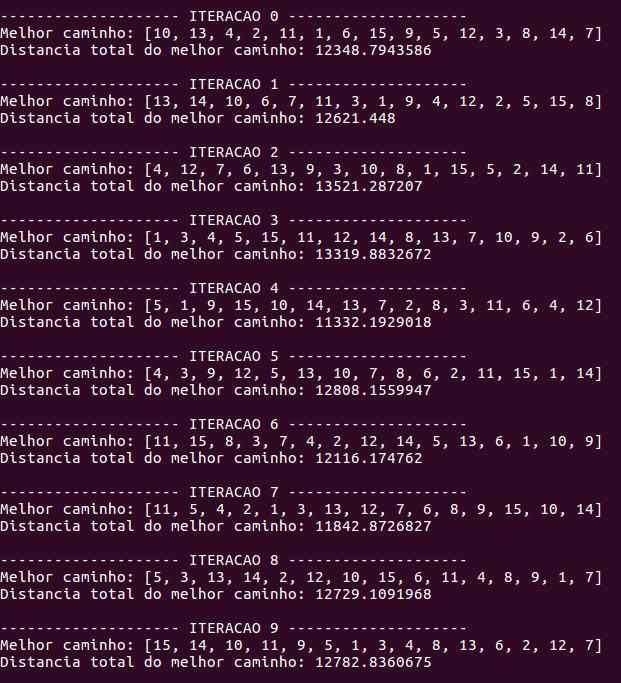
\includegraphics[scale=0.6]{Figures/m15-1-1.png}
		\end{figure}

		\newpage
		
		\begin{figure}[!h]
			\centering
			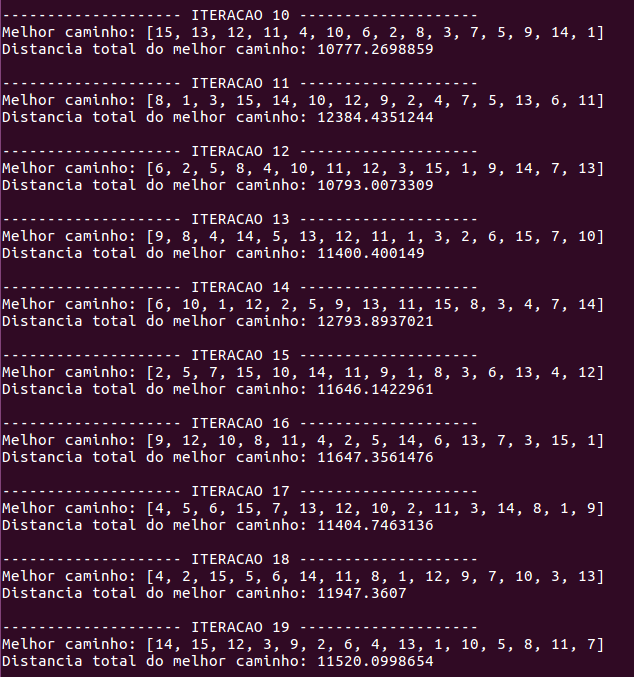
\includegraphics[scale=0.6]{Figures/m15-1-2.png}
		\end{figure}

		\newpage
		
		\begin{figure}[!h]
			\centering
			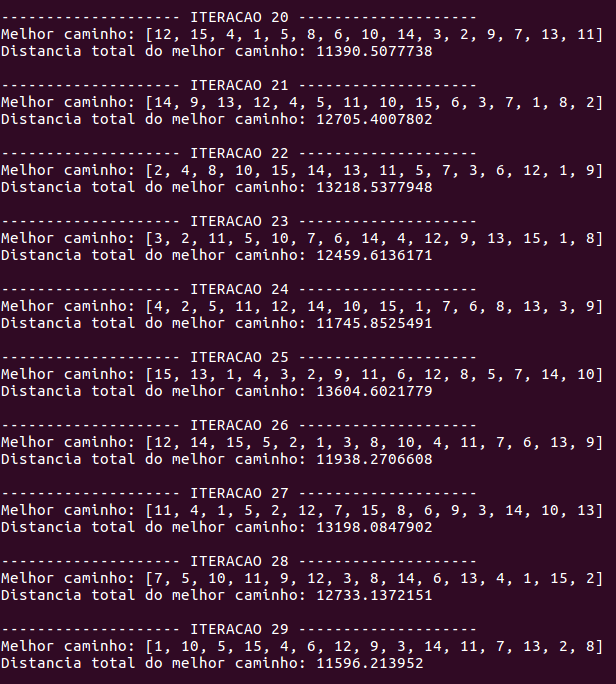
\includegraphics[scale=0.6]{Figures/m15-1-3.png}
		\end{figure}

		\newpage
		
		\begin{figure}[!h]
			\centering
			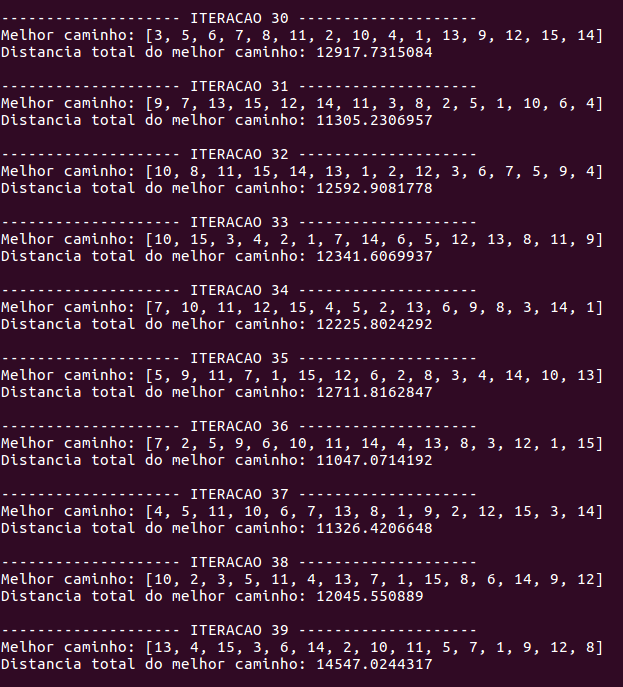
\includegraphics[scale=0.6]{Figures/m15-1-4.png}
		\end{figure}

		\newpage
		
		\begin{figure}[!h]
			\centering
			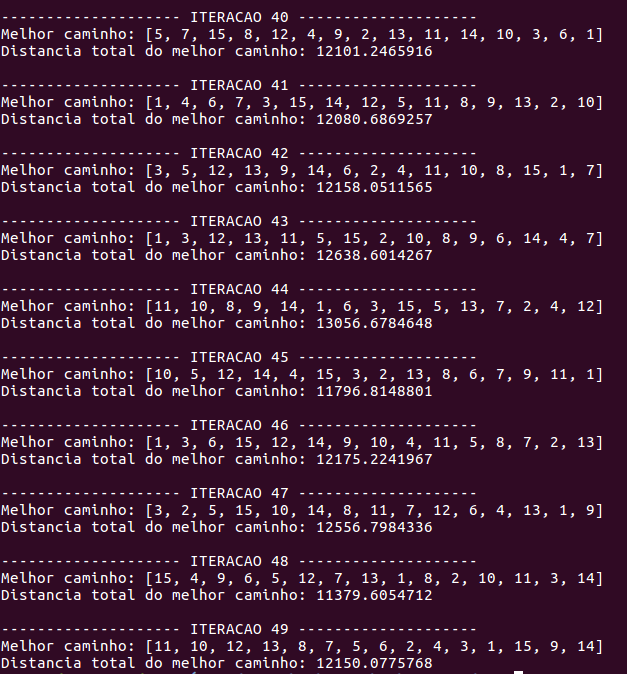
\includegraphics[scale=0.6]{Figures/m15-1-5.png}
		\end{figure}
		
		\newpage
		
		\subsubsection{Segunda configuração}
		 	Para este experimento foi utilizada a seguinte configuração:

		 	\begin{itemize}
				\item Número de repetições: 50
				\item Número máximo de iterações para achar o melhor caminho: 1000
				\item Quantidade de feromôneo depositado por cada formiga: 1
				\item Taxa de evaporação do feromônio: 0.8
			\end{itemize}

		\newpage	

		\begin{figure}[!h]
			\centering
			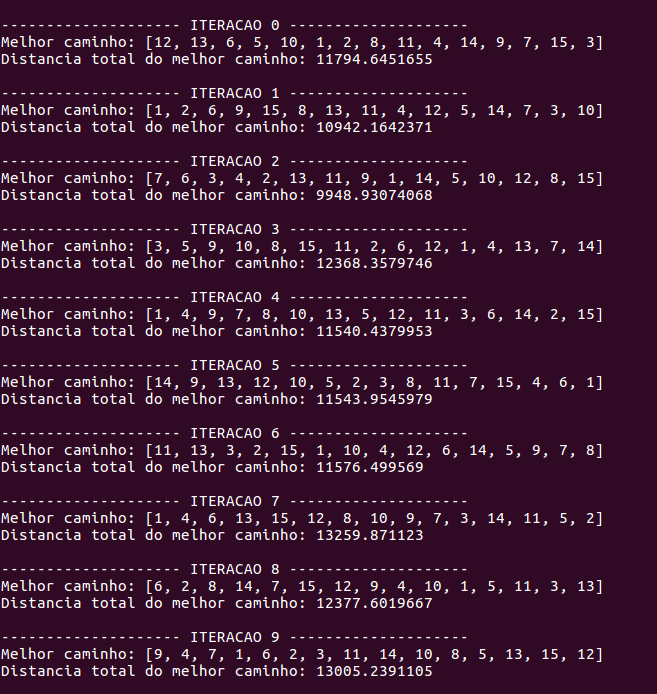
\includegraphics[scale=0.6]{Figures/m15-2-1.png}
		\end{figure}

		\newpage
		
		\begin{figure}[!h]
			\centering
			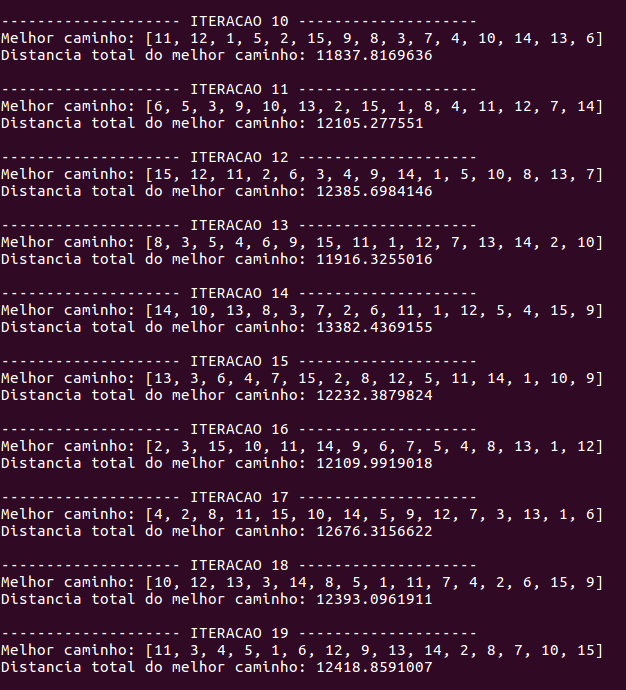
\includegraphics[scale=0.6]{Figures/m15-2-2.png}
		\end{figure}

		\newpage
		
		\begin{figure}[!h]
			\centering
			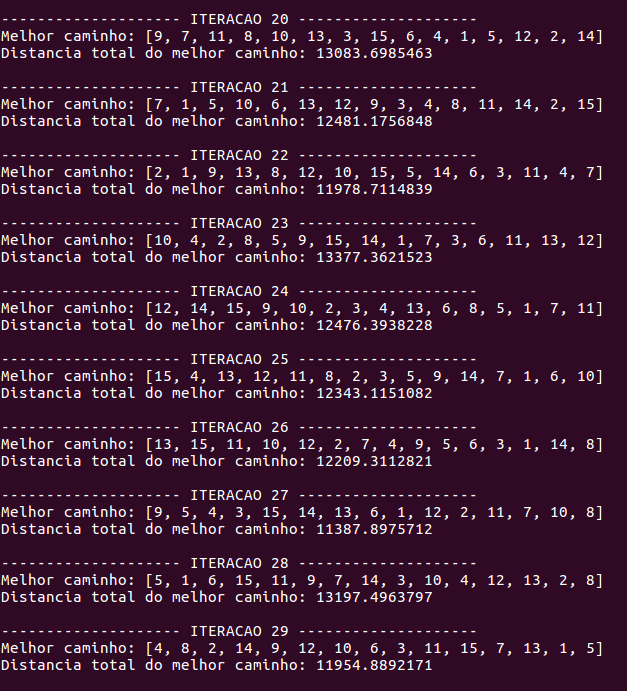
\includegraphics[scale=0.6]{Figures/m15-2-3.png}
		\end{figure}

		\newpage
		
		\begin{figure}[!h]
			\centering
			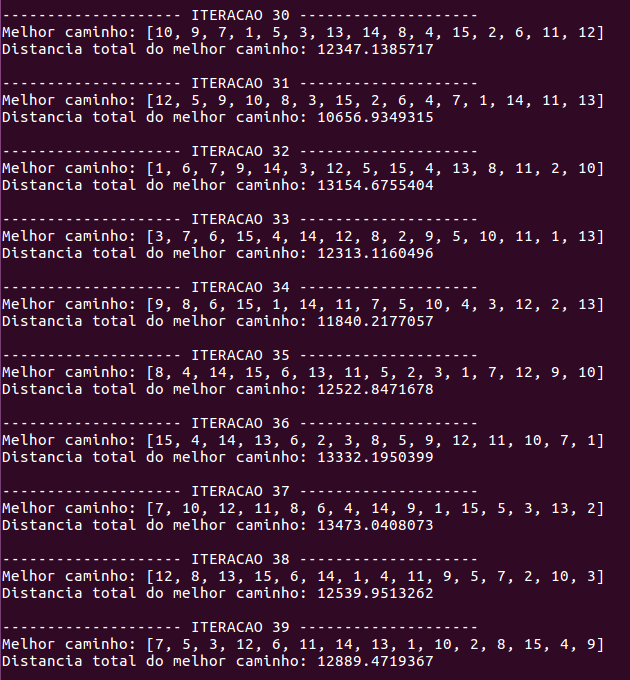
\includegraphics[scale=0.6]{Figures/m15-2-4.png}
		\end{figure}

		\newpage
		
		\begin{figure}[!h]
			\centering
			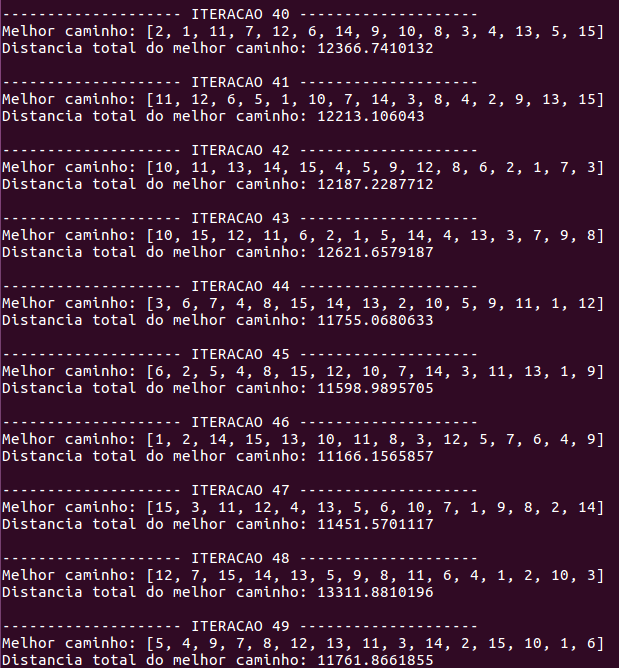
\includegraphics[scale=0.6]{Figures/m15-2-5.png}
		\end{figure}

		\newpage	

	\subsection{M29}
			Neste exercício é fornecido as coordenadas de 29 cidades diferentes.	
		\subsubsection{Primeira configuração}
		 	Para este experimento foi utilizada a seguinte configuração:

		 	\begin{itemize}
				\item Número de repetições: 50
				\item Número máximo de iterações para achar o melhor caminho: 100
				\item Quantidade de feromôneo depositado por cada formiga: 1
				\item Taxa de evaporação do feromônio: 0.5
			\end{itemize}


		\newpage 	

		\begin{figure}[!h]
			\centering
			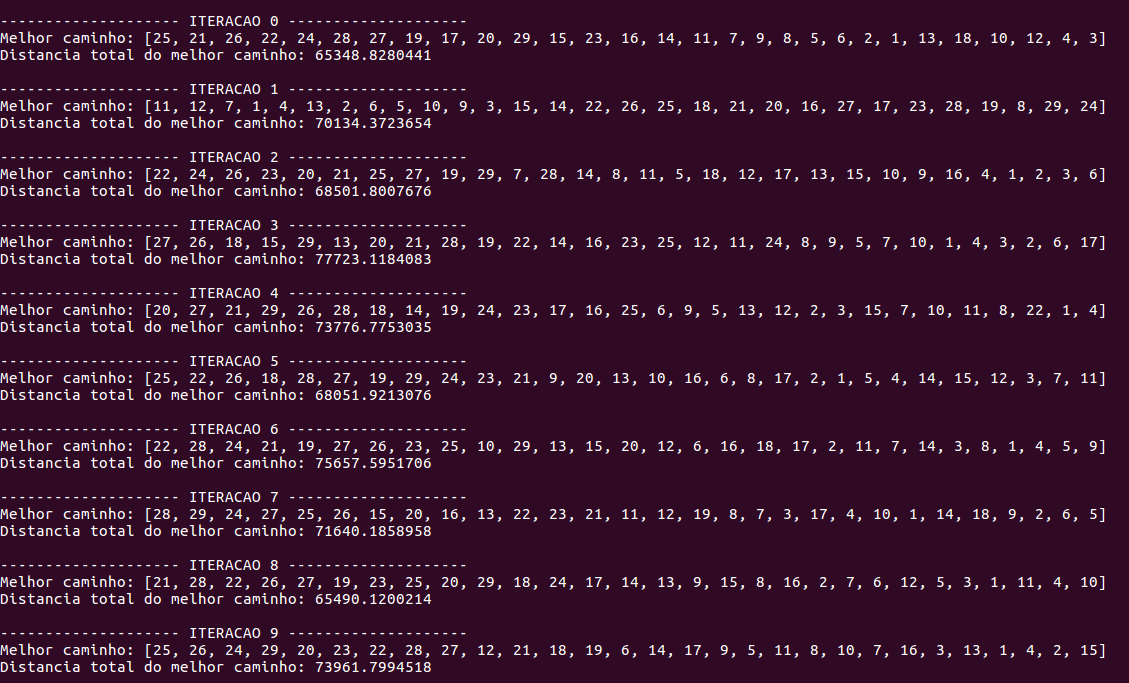
\includegraphics[scale=0.4]{Figures/m29-1-1.png}
		\end{figure}

		\newpage

		\begin{figure}[!h]
			\centering
			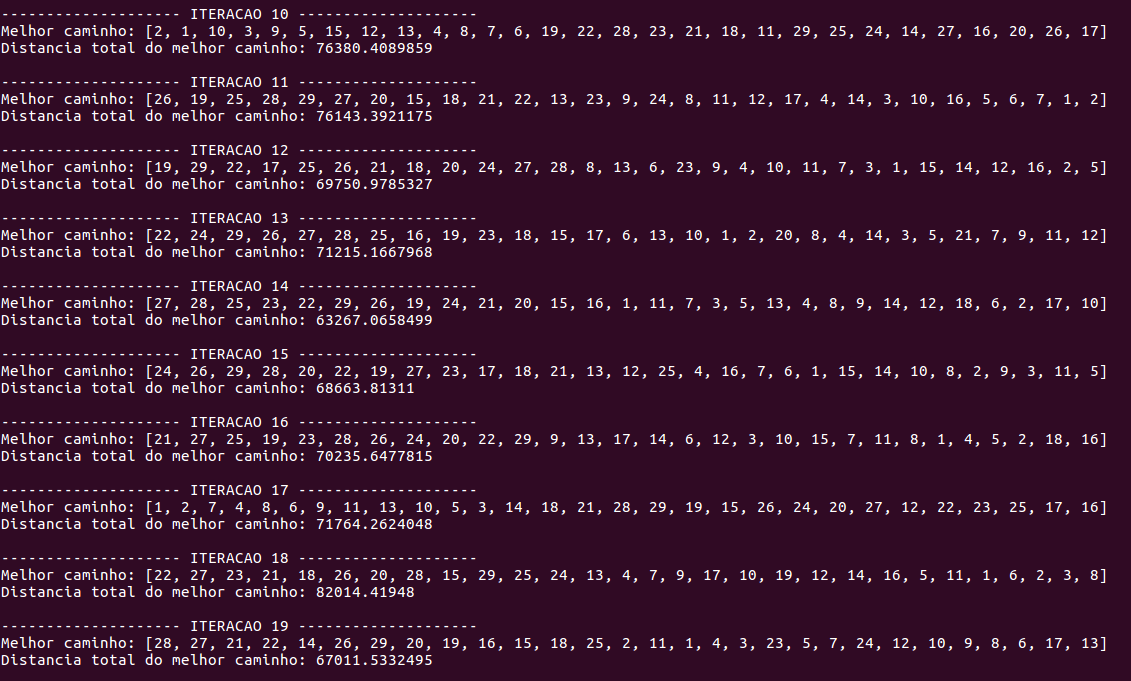
\includegraphics[scale=0.4]{Figures/m29-1-2.png}
		\end{figure}

		\newpage

		\begin{figure}[!h]
			\centering
			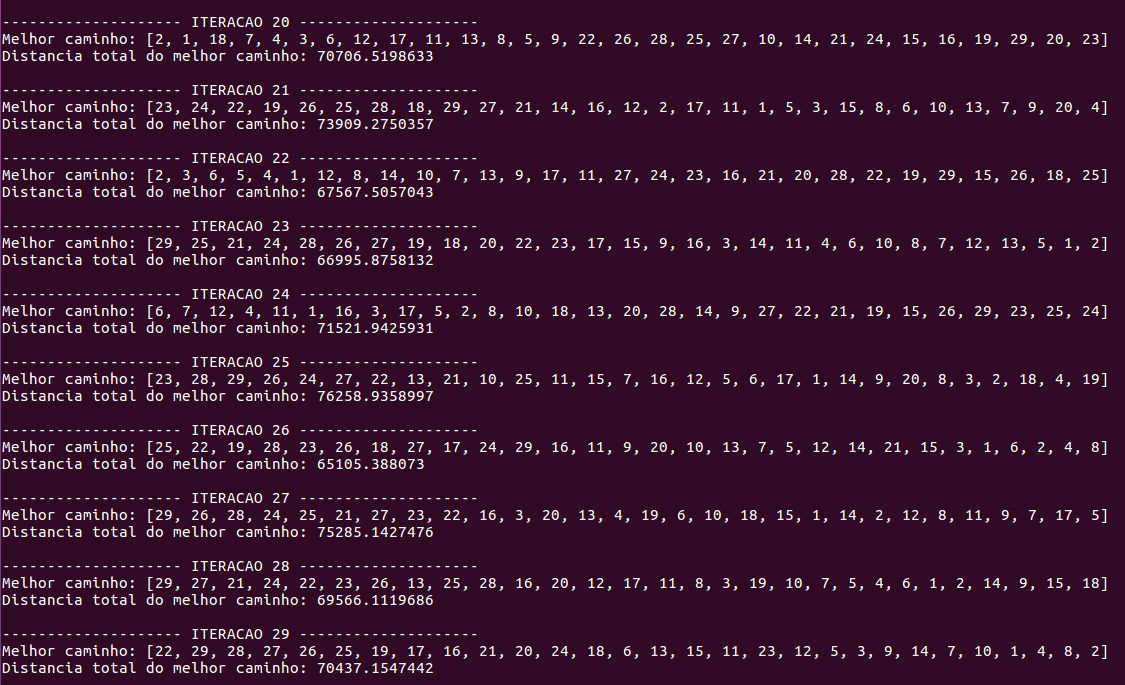
\includegraphics[scale=0.4]{Figures/m29-1-3.png}
		\end{figure}

		\newpage

		\begin{figure}[!h]
			\centering
			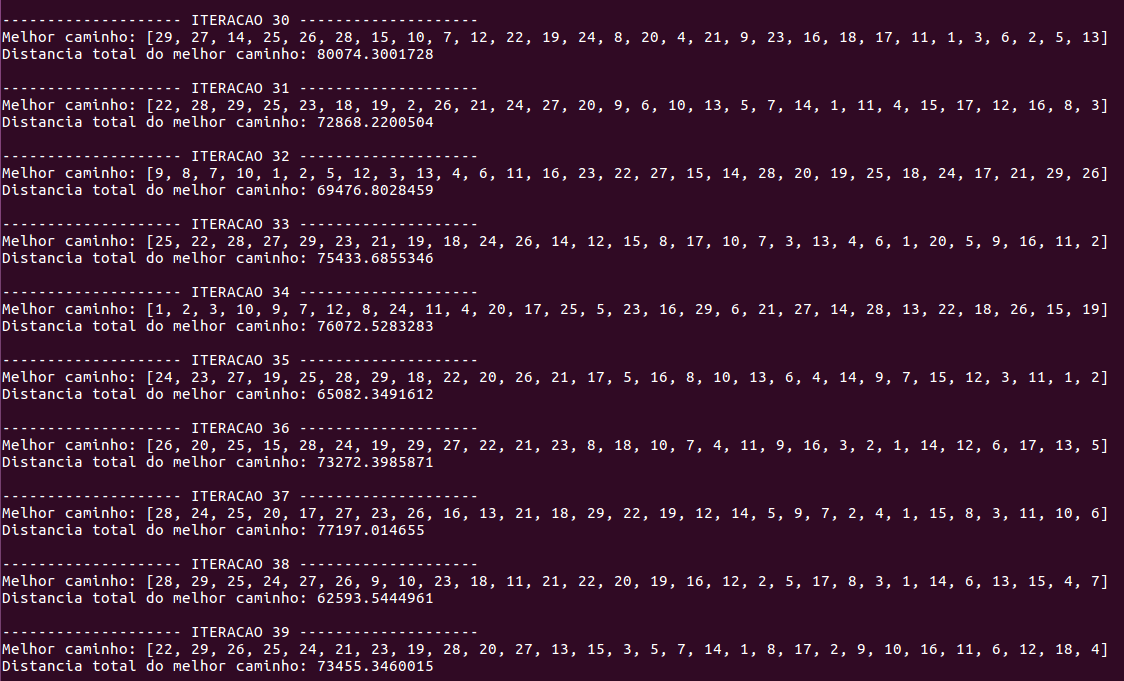
\includegraphics[scale=0.4]{Figures/m29-1-4.png}
		\end{figure}

		\newpage

		\begin{figure}[!h]
			\centering
			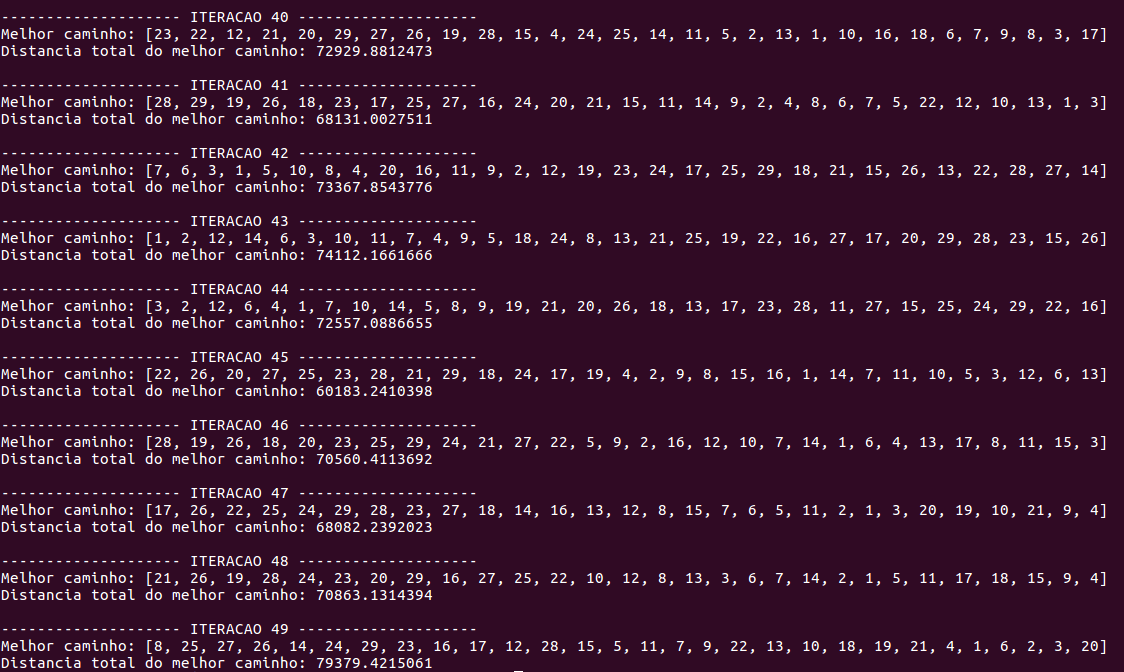
\includegraphics[scale=0.4]{Figures/m29-1-5.png}
		\end{figure}
		
		\newpage
		
		\subsubsection{Segunda configuração}
		 	Para este experimento foi utilizada a seguinte configuração:

		 	\begin{itemize}
				\item Número de repetições: 50
				\item Número máximo de iterações para achar o melhor caminho: 10
				\item Quantidade de feromôneo depositado por cada formiga: 1
				\item Taxa de evaporação do feromônio: 0.8
			\end{itemize}

		\newpage

		\begin{figure}[!h]
			\centering
			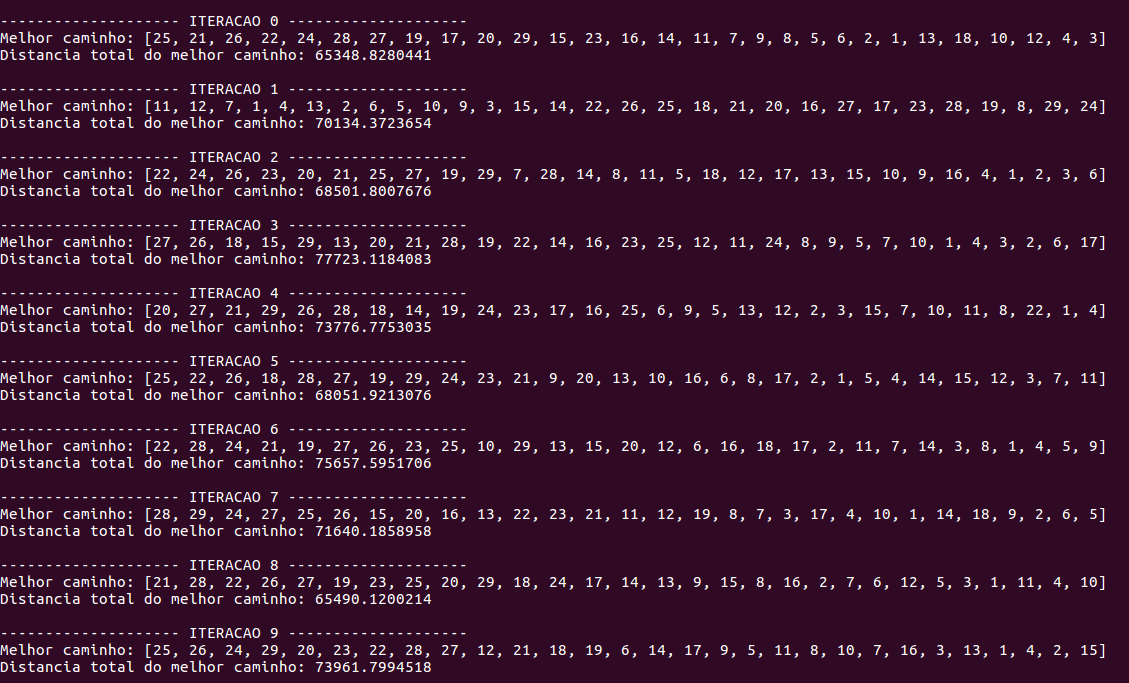
\includegraphics[scale=0.4]{Figures/m29-1-1.png}
		\end{figure}

		\newpage

		\begin{figure}[!h]
			\centering
			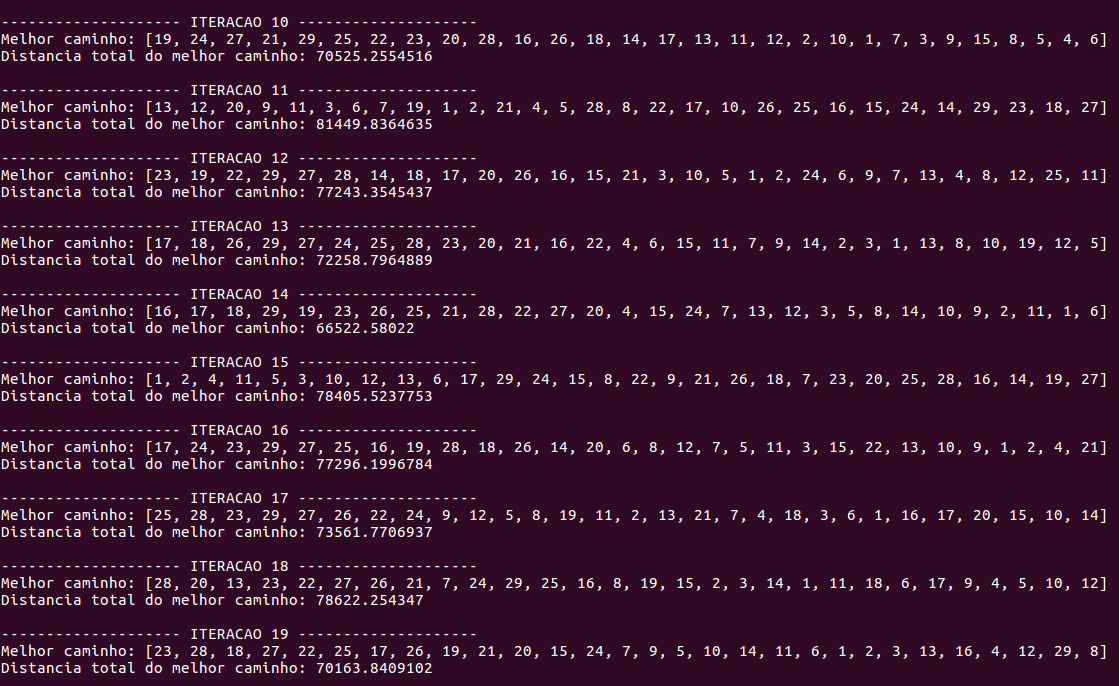
\includegraphics[scale=0.4]{Figures/m29-2-2.png}
		\end{figure}

		\newpage

		\begin{figure}[!h]
			\centering
			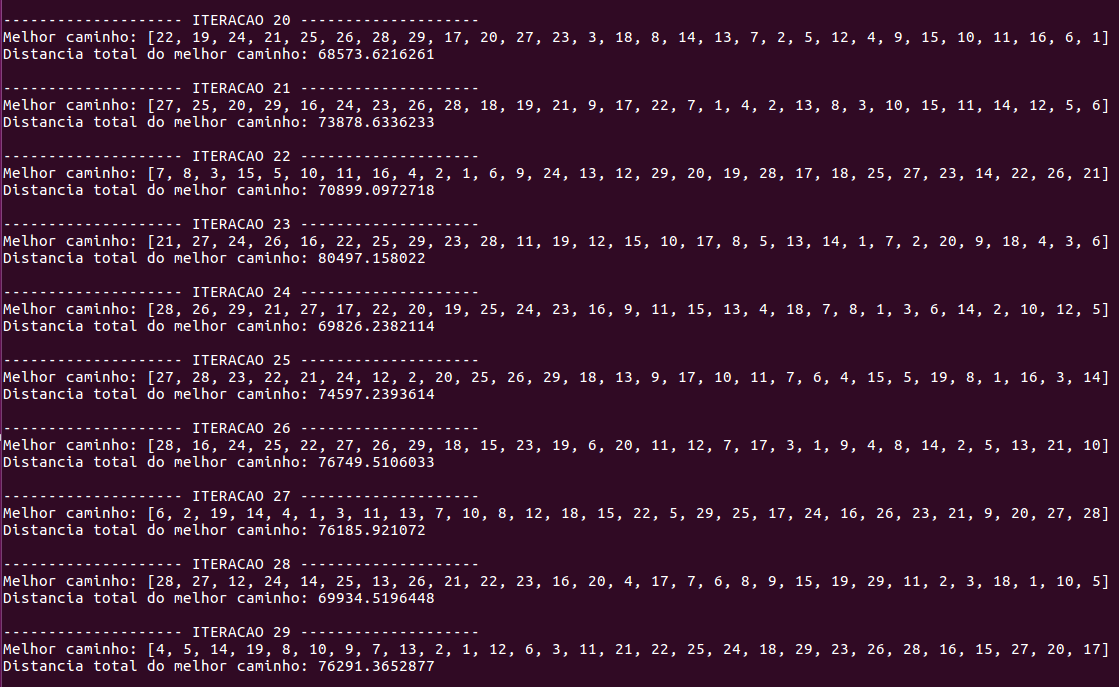
\includegraphics[scale=0.4]{Figures/m29-2-3.png}
		\end{figure}

		\newpage

		\begin{figure}[!h]
			\centering
			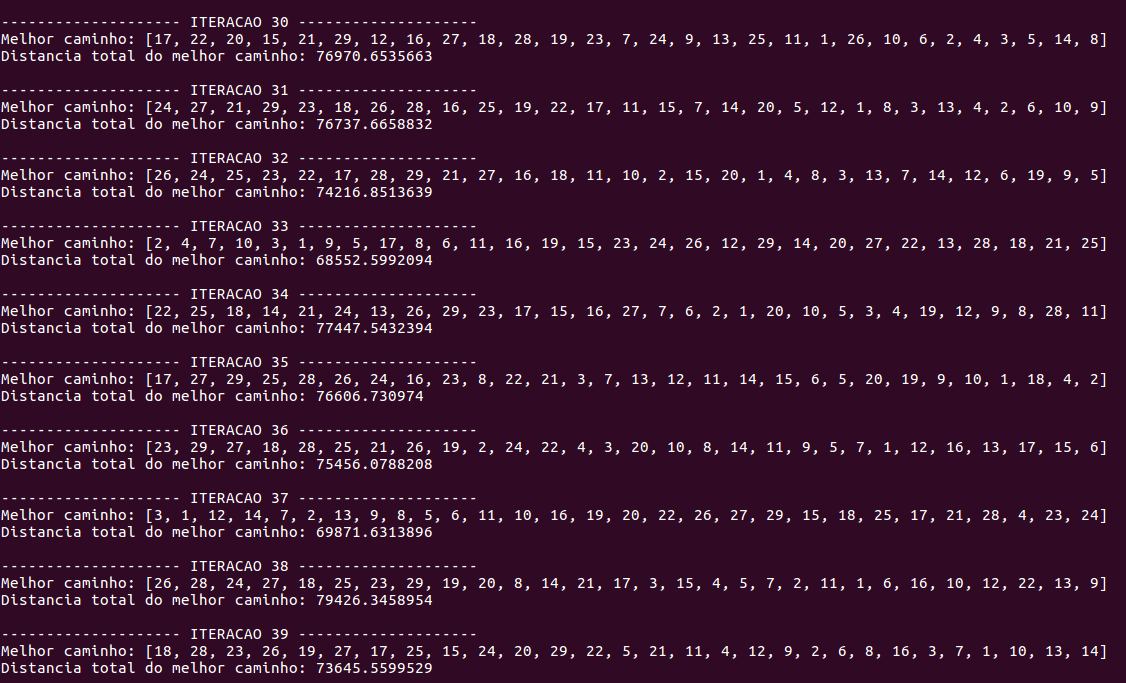
\includegraphics[scale=0.4]{Figures/m29-2-4.png}
		\end{figure}

		\newpage

		\begin{figure}[!h]
			\centering
			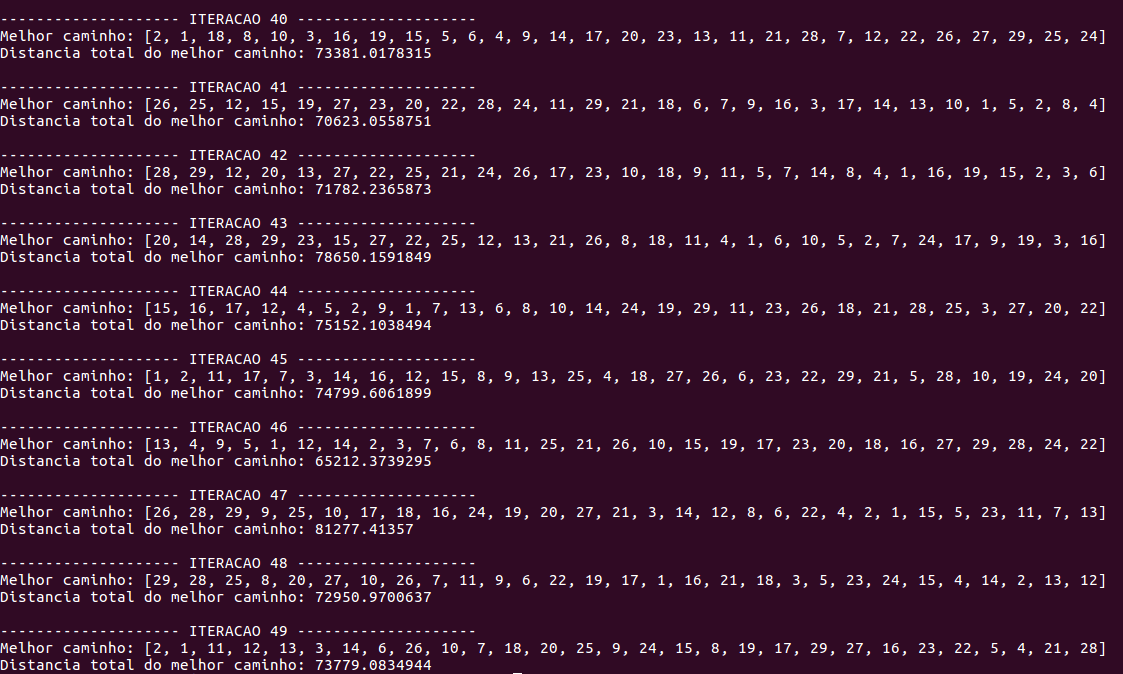
\includegraphics[scale=0.4]{Figures/m29-2-5.png}
		\end{figure}

		\newpage		
	
	\subsection{M38}
			Neste exercício é fornecido as coordenadas de 38 cidades diferentes.	
		\subsubsection{Primeira configuração}
		 	Para este experimento foi utilizada a seguinte configuração:

		 	\begin{itemize}
				\item Número de repetições: 50
				\item Número máximo de iterações para achar o melhor caminho: 100
				\item Quantidade de feromôneo depositado por cada formiga: 1
				\item Taxa de evaporação do feromônio: 0.5
			\end{itemize}

		\newpage

		\begin{figure}[!h]
			\centering
			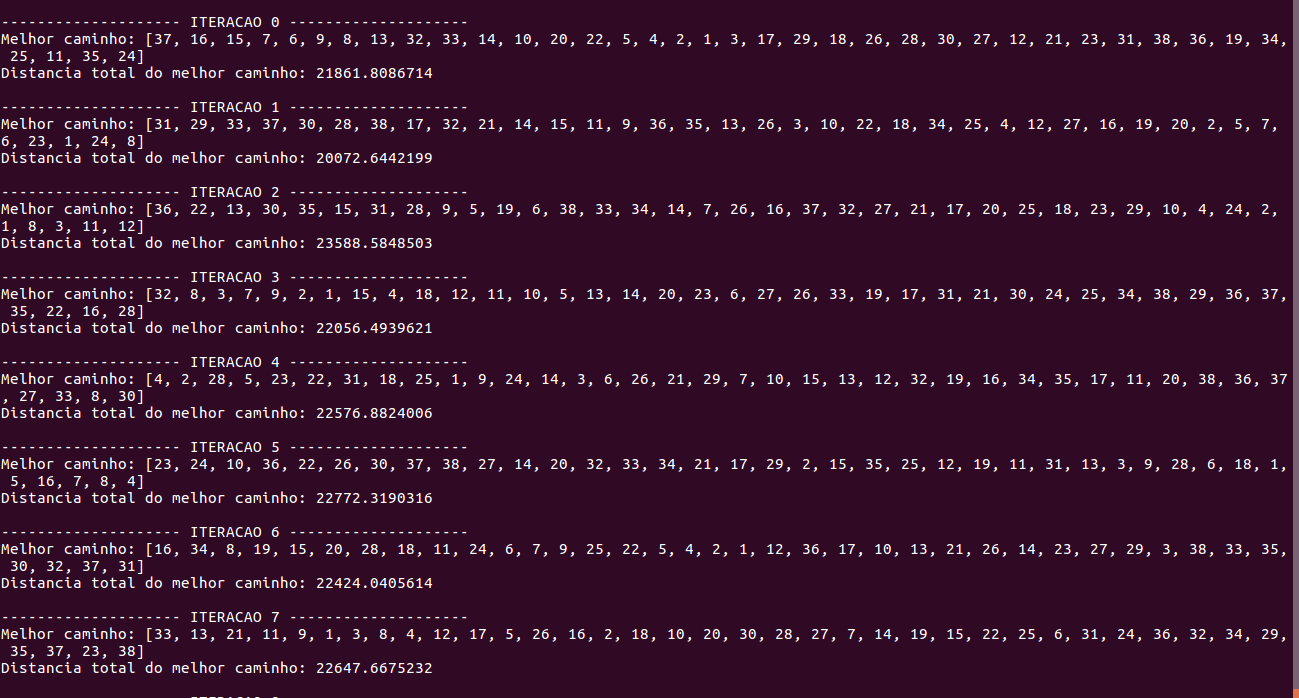
\includegraphics[scale=0.3]{Figures/m38-1-1.png}
		\end{figure}

		\newpage

		\begin{figure}[!h]
			\centering
			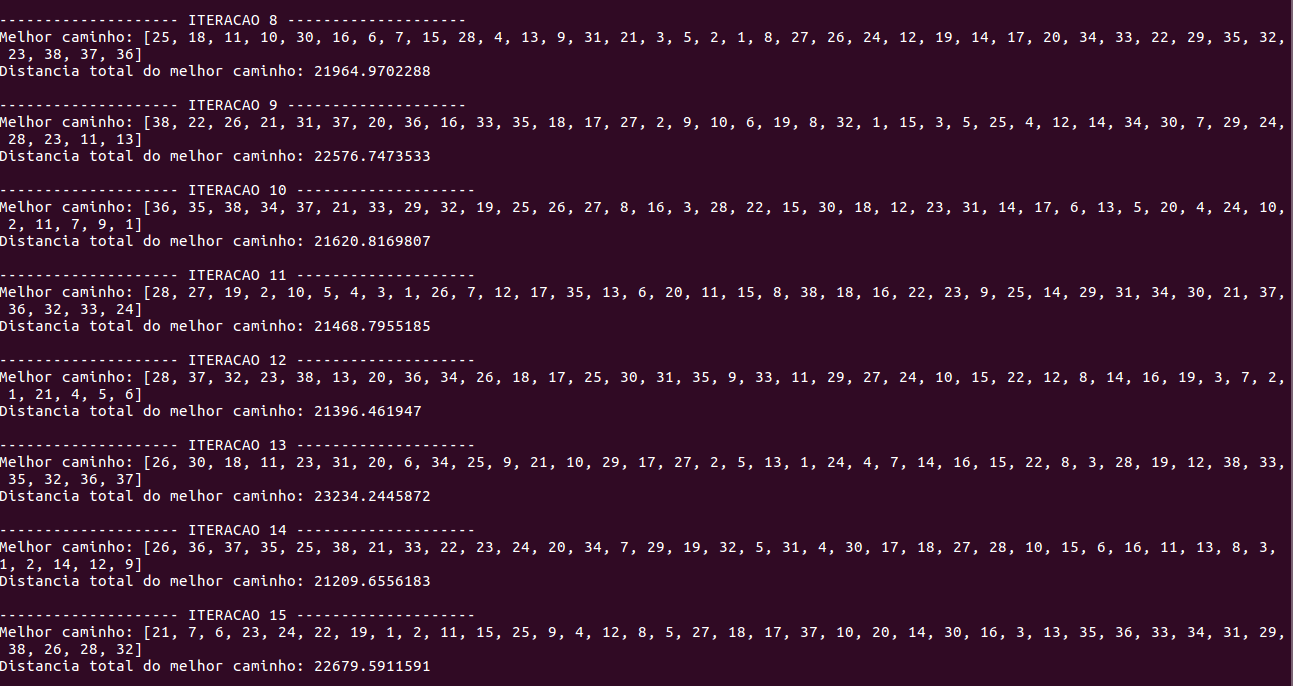
\includegraphics[scale=0.3]{Figures/m38-1-2.png}
		\end{figure}

		\newpage

		\begin{figure}[!h]
			\centering
			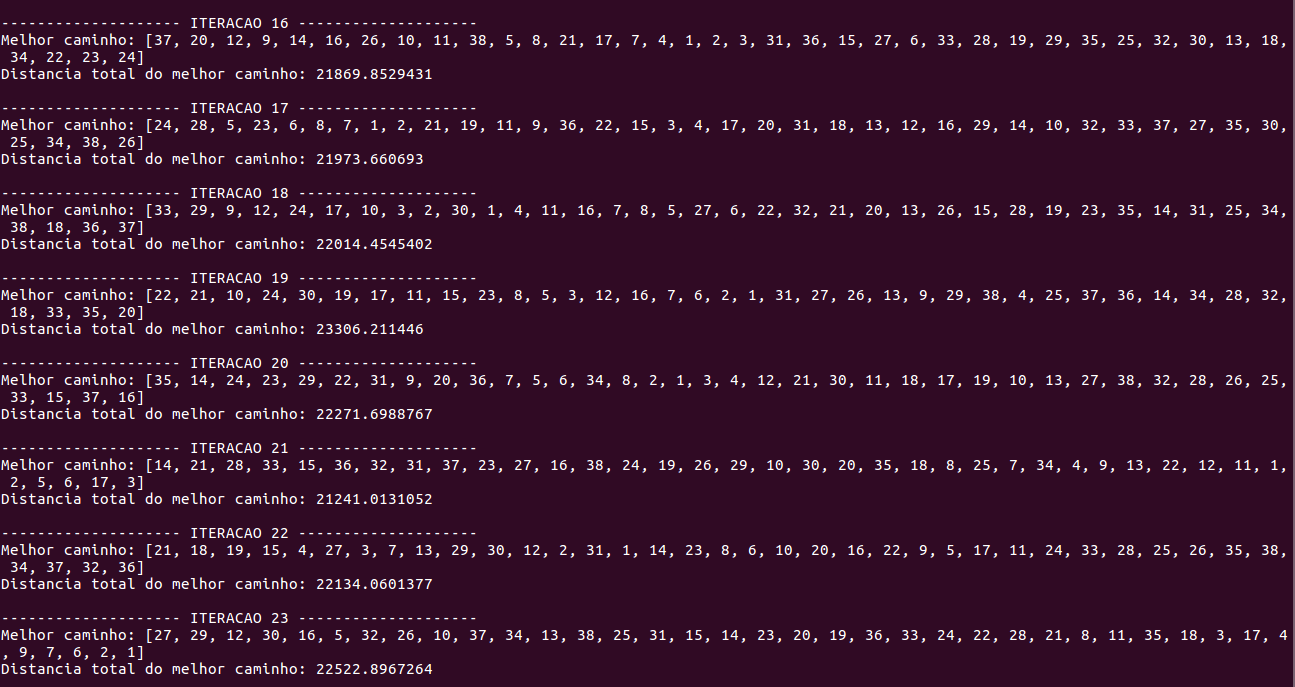
\includegraphics[scale=0.3]{Figures/m38-1-3.png}
		\end{figure}

		\newpage

		\begin{figure}[!h]
			\centering
			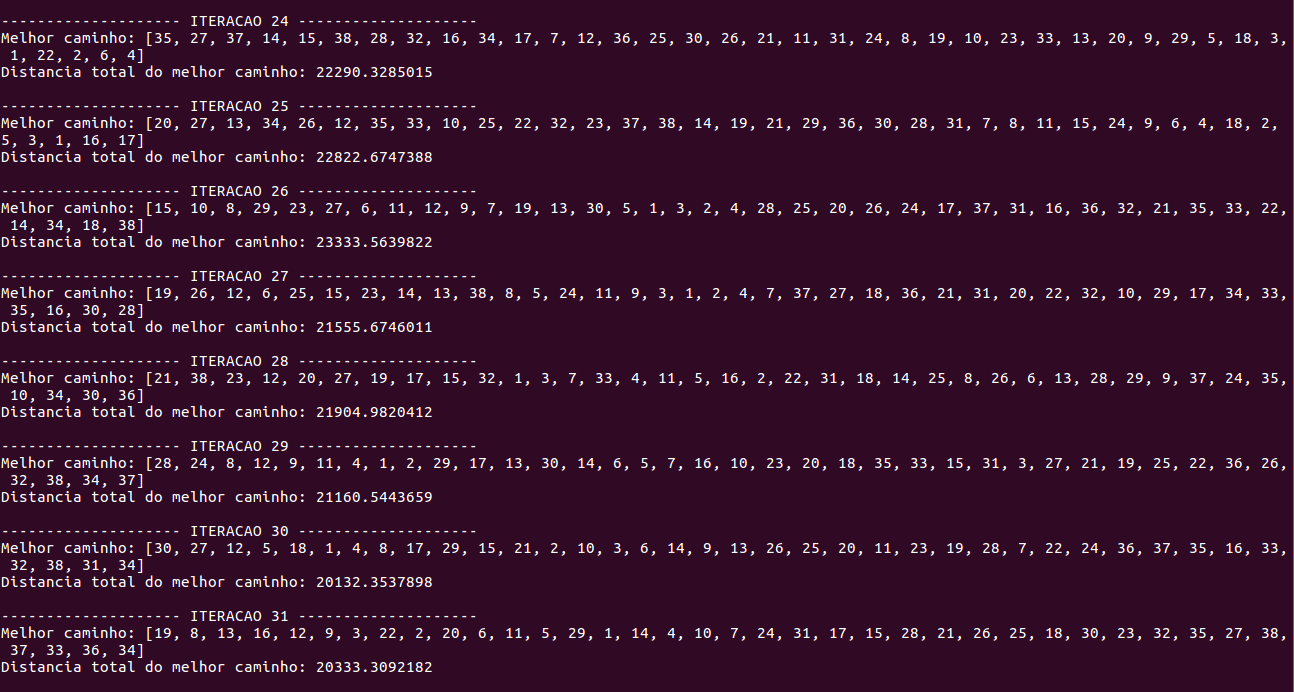
\includegraphics[scale=0.3]{Figures/m38-1-4.png}
		\end{figure}

		\newpage

		\begin{figure}[!h]
			\centering
			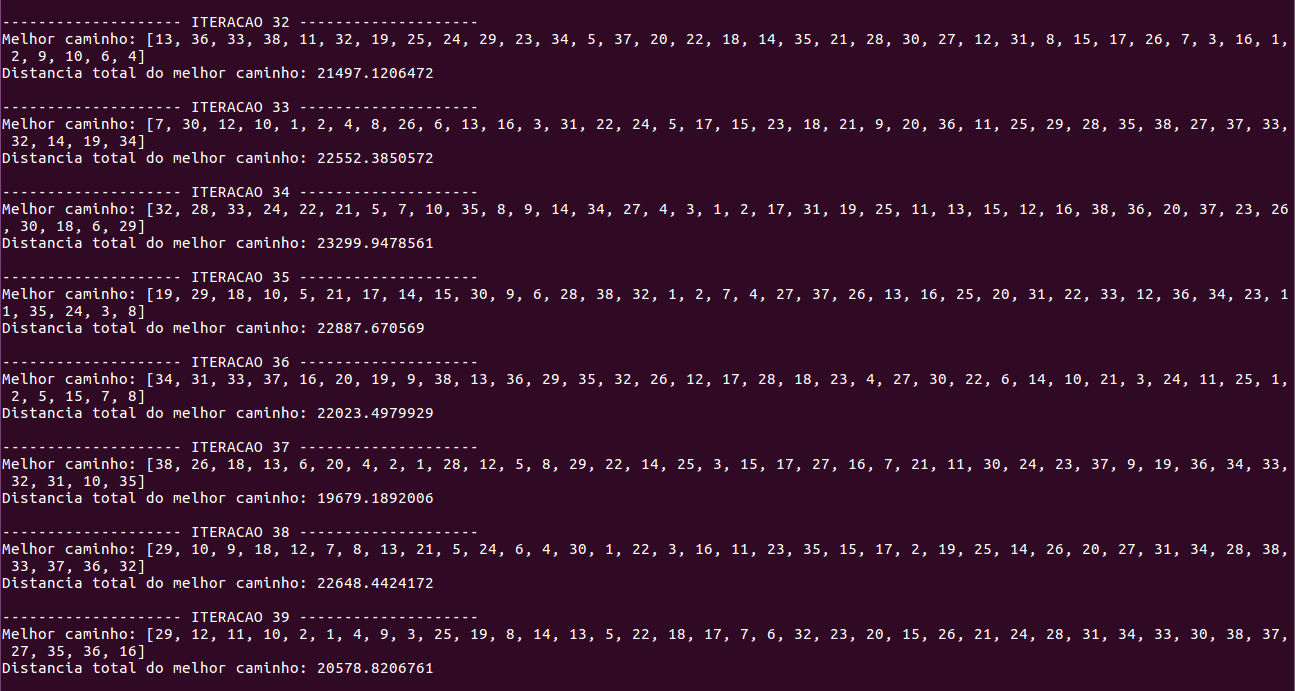
\includegraphics[scale=0.3]{Figures/m38-1-5.png}
		\end{figure}

		\newpage

		\begin{figure}[!h]
			\centering
			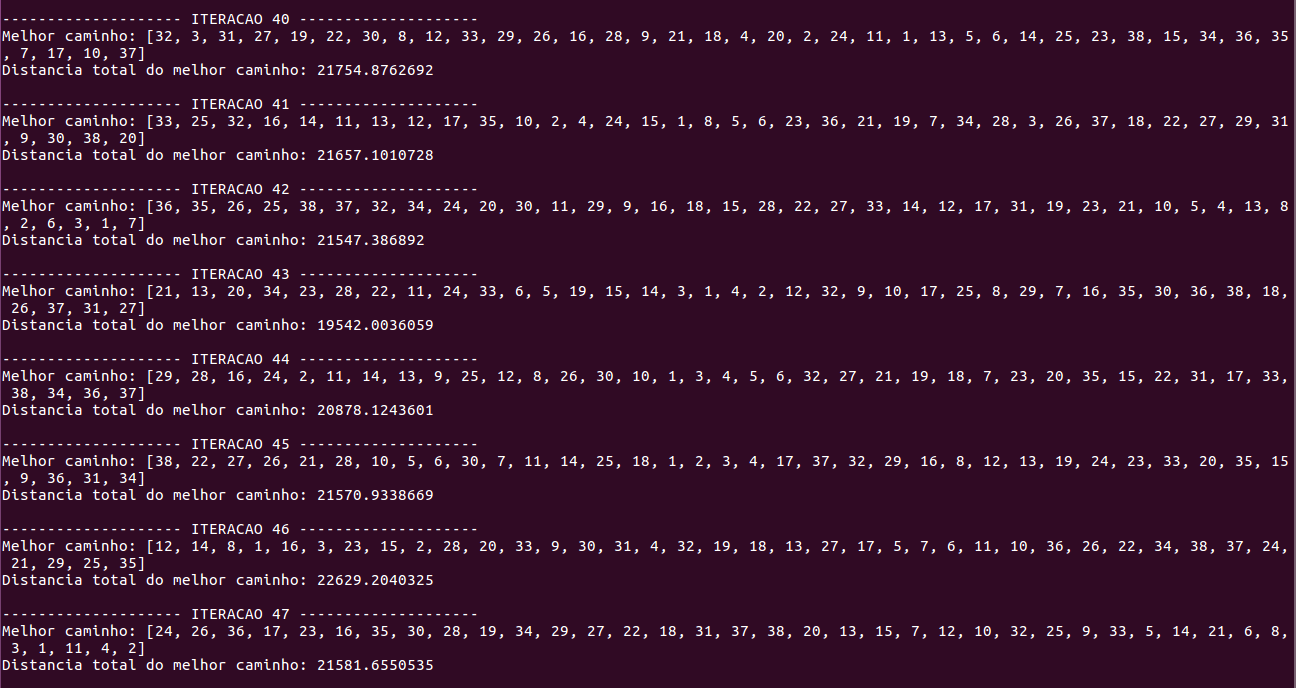
\includegraphics[scale=0.3]{Figures/m38-1-6.png}
		\end{figure}

		\newpage

		\begin{figure}[!h]
			\centering
			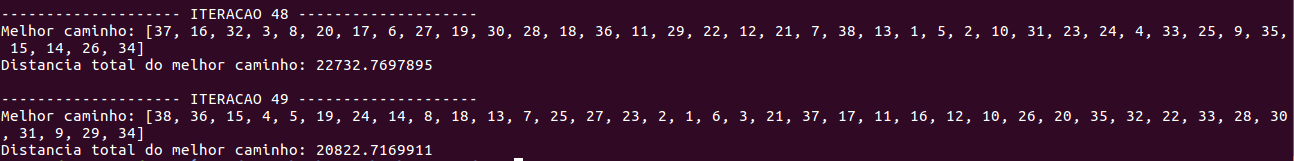
\includegraphics[scale=0.3]{Figures/m38-1-7.png}
		\end{figure}
		
		\newpage
		
		\subsubsection{Segunda configuração}
		 	Para este experimento foi utilizada a seguinte configuração:

		 	\begin{itemize}
				\item Número de repetições: 50
				\item Número máximo de iterações para achar o melhor caminho: 10
				\item Quantidade de feromôneo depositado por cada formiga: 1
				\item Taxa de evaporação do feromônio: 0.8
			\end{itemize}

		\newpage

		\begin{figure}[!h]
			\centering
			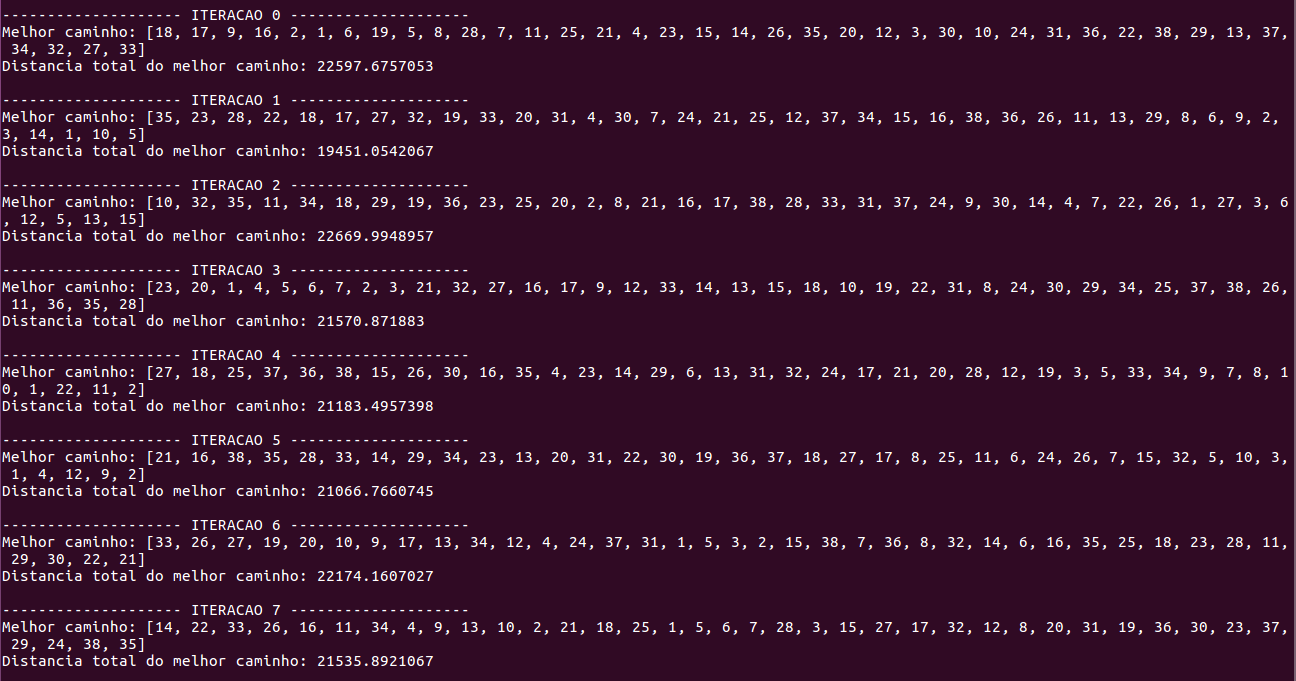
\includegraphics[scale=0.3]{Figures/m38-2-1.png}
		\end{figure}

		\newpage

		\begin{figure}[!h]
			\centering
			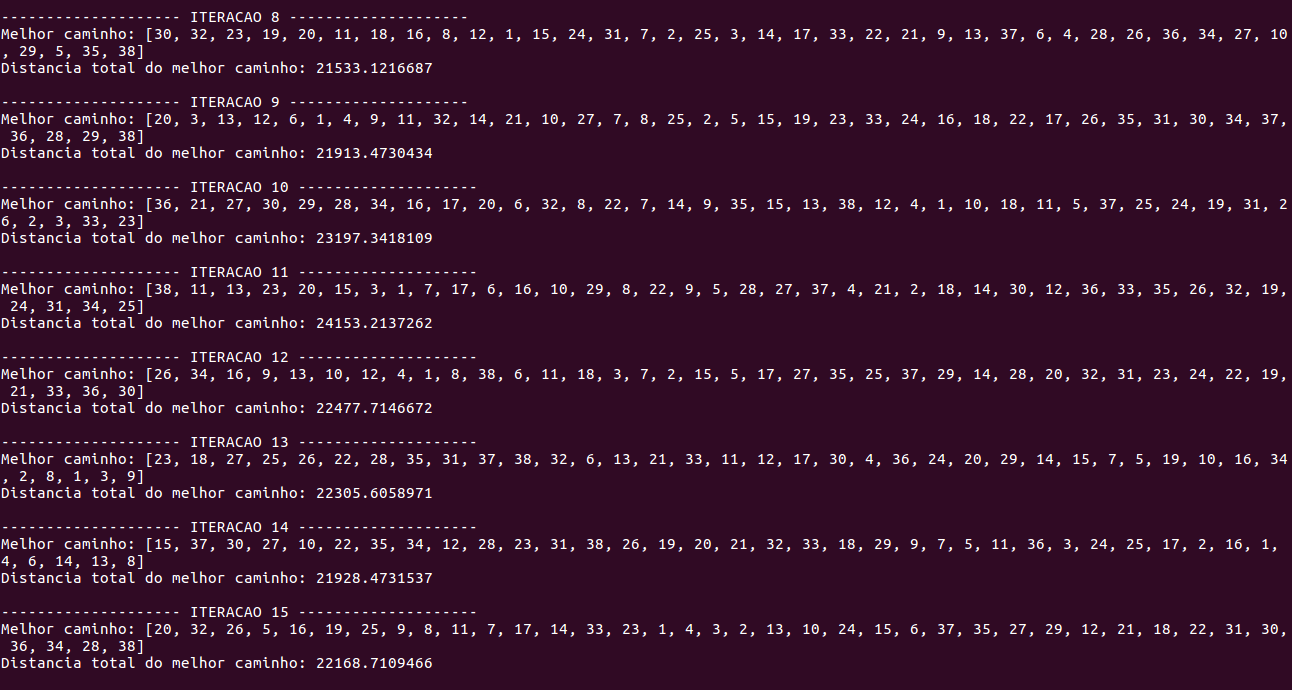
\includegraphics[scale=0.3]{Figures/m38-2-2.png}
		\end{figure}

		\newpage

		\begin{figure}[!h]
			\centering
			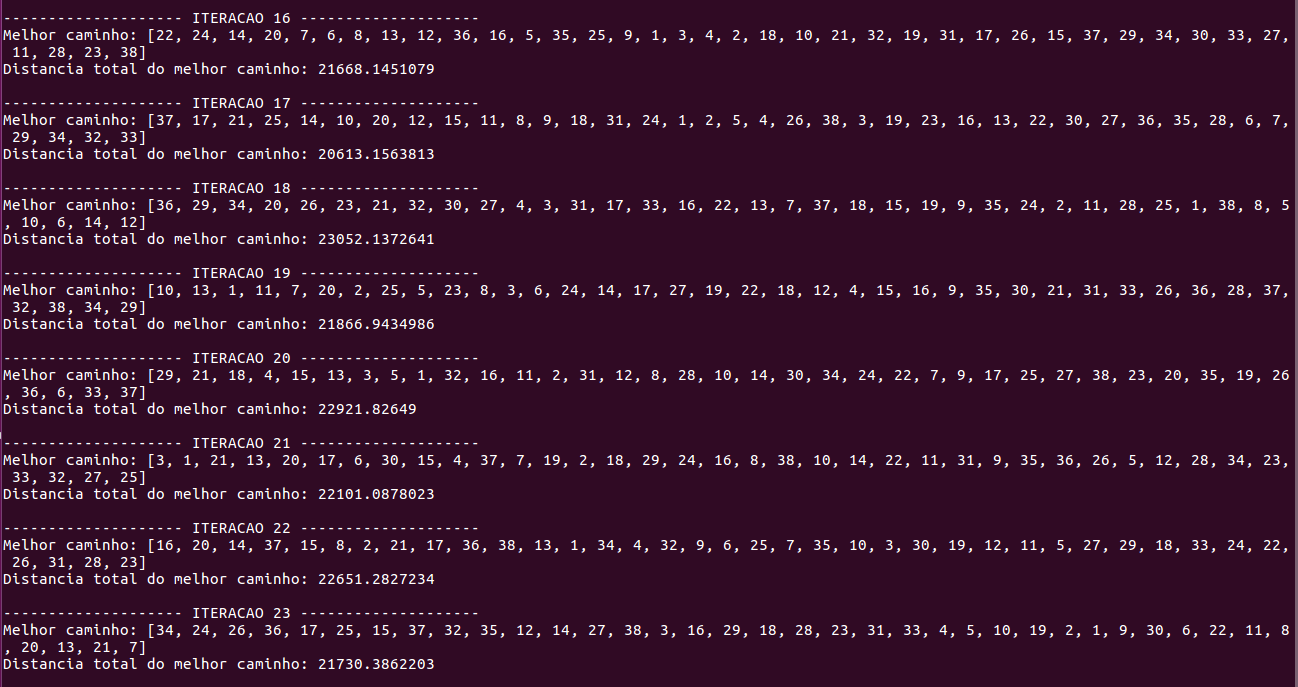
\includegraphics[scale=0.3]{Figures/m38-2-3.png}
		\end{figure}

		\newpage

		\begin{figure}[!h]
			\centering
			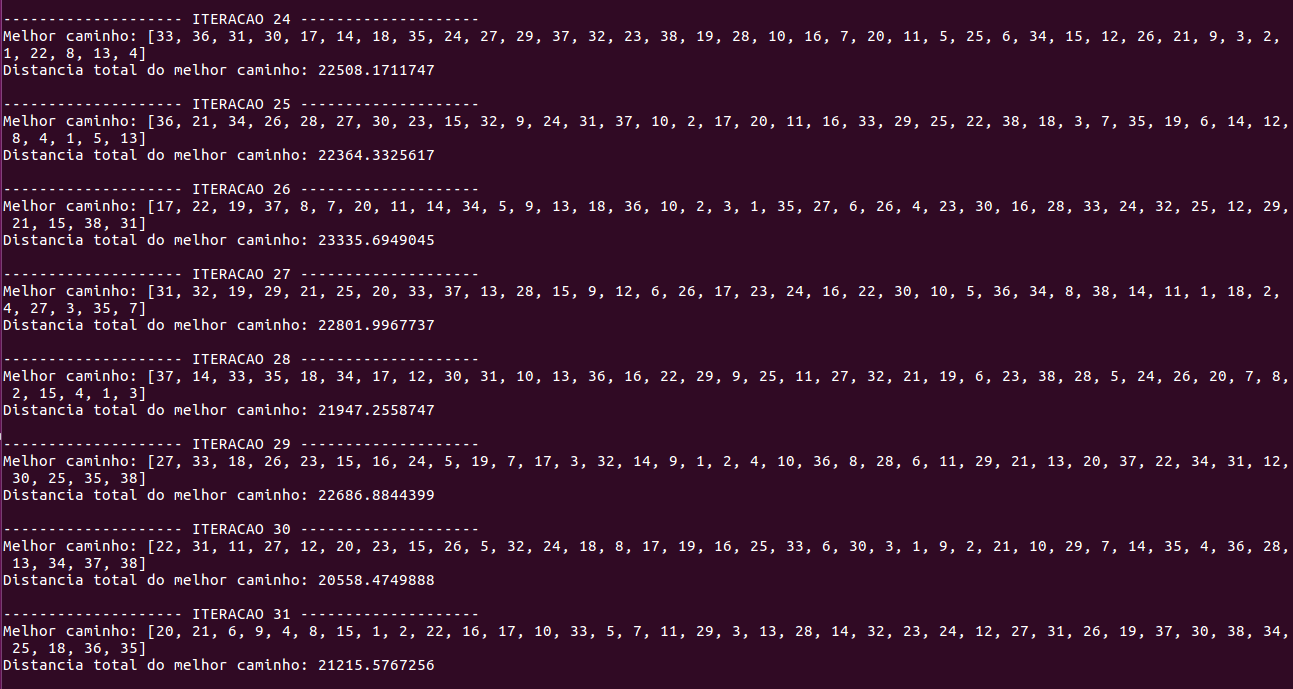
\includegraphics[scale=0.3]{Figures/m38-2-4.png}
		\end{figure}

		\newpage

		\begin{figure}[!h]
			\centering
			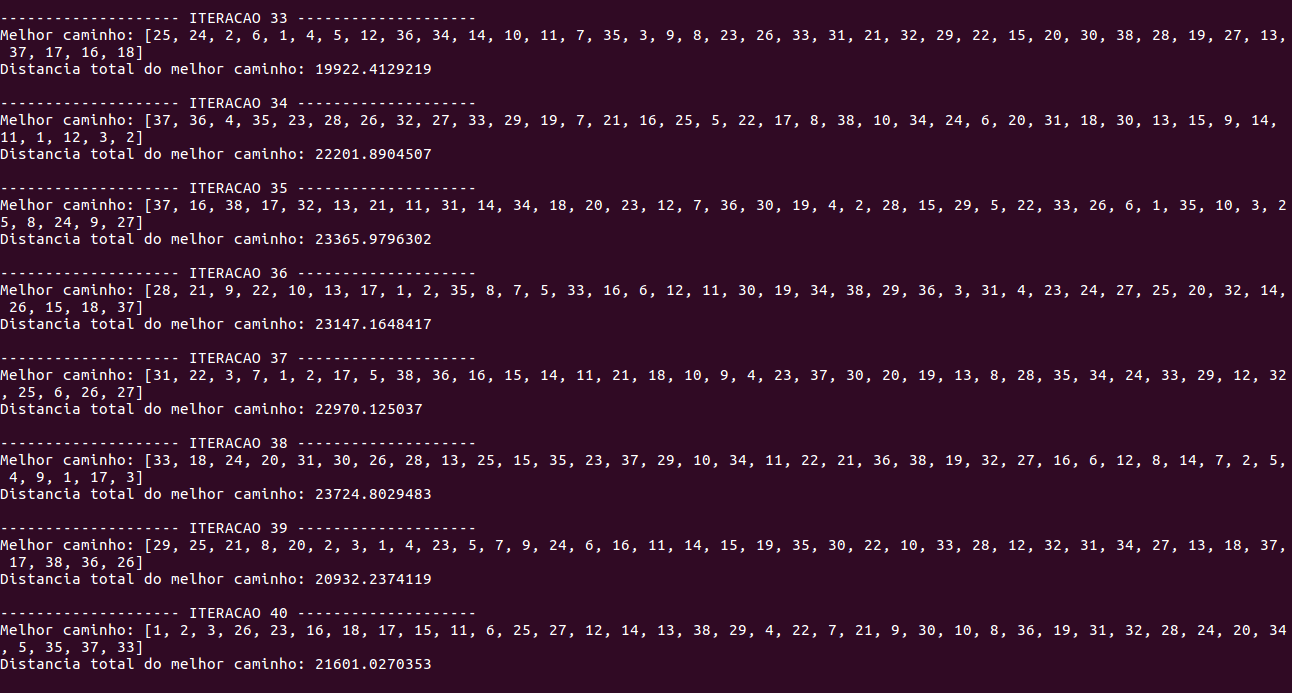
\includegraphics[scale=0.3]{Figures/m38-2-5.png}
		\end{figure}

		\newpage

		\begin{figure}[!h]
			\centering
			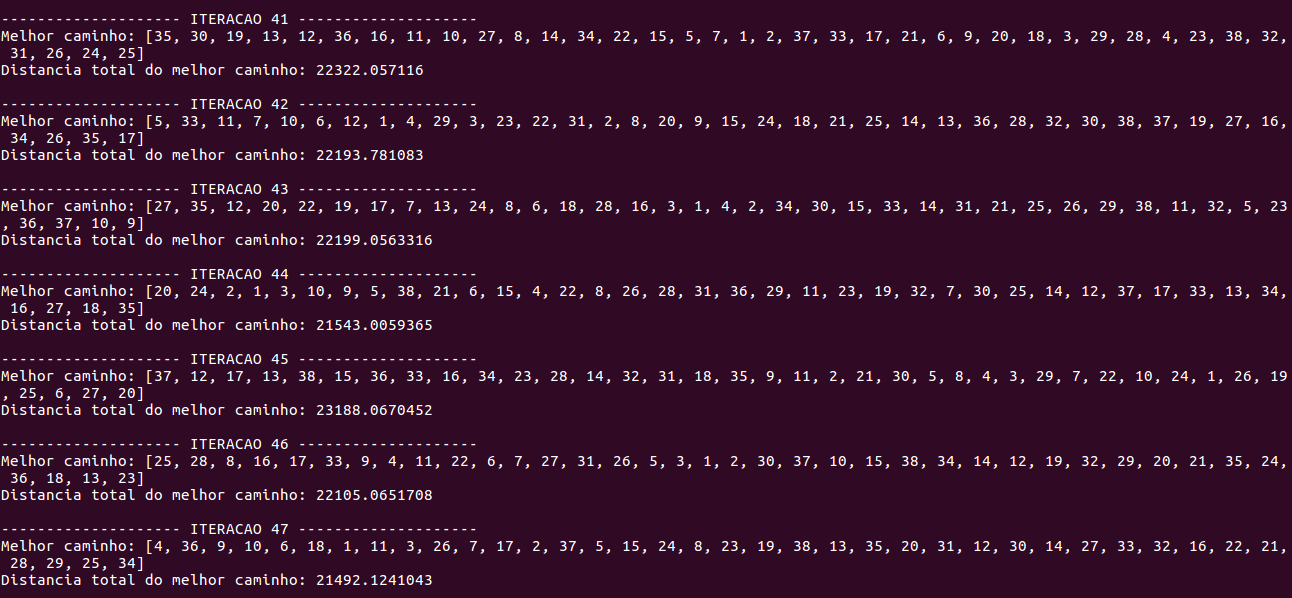
\includegraphics[scale=0.3]{Figures/m38-2-6.png}
		\end{figure}

		\newpage

		\begin{figure}[!h]
			\centering
			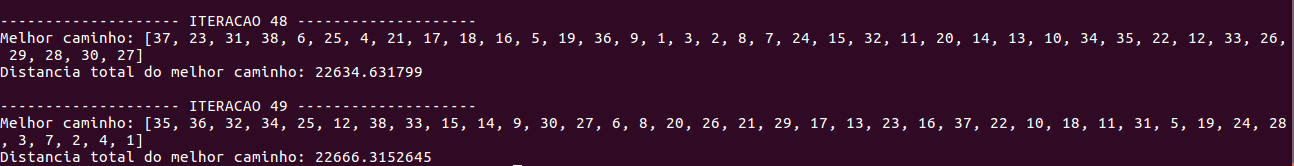
\includegraphics[scale=0.3]{Figures/m38-2-7.png}
		\end{figure}
\end{document}
